\section{Role of mechanical twinning in plastic deformation of HCP metals.}
Hexagonal Closed Packed lattice itself causes significant anisotropy which has effect on deformation mechanisms. Due to this, hexagonal close-packed metals have the challenge of activating slip along the $\langle c \rangle$-axis at low temperatures and/or high strain rates. Since 4 independent basal slip systems are not enough to accommodate an arbitrary deformation fulfilling von Mises criterion \cite{taylor1938plastic}, twinning will take the role to mediate the plastic deformation in the $\langle c \rangle$-axis taking the role of pyramidal slip systems which are difficult to activate.
Figure \ref{Twin_slip_MG_CRSS} gives the Critical Resolved Shear Stress (CRSS) values. CRSS values quantitatively informs how easy or difficult a particular deformation mode to mediate plastic deformation. The lack of available deformation mechanisms can be qualitatively observed by presence of strong basal texture \cite{Yoo1981409} in cold worked Mg alloys. 
\begin{figure}[H]
    \centering
    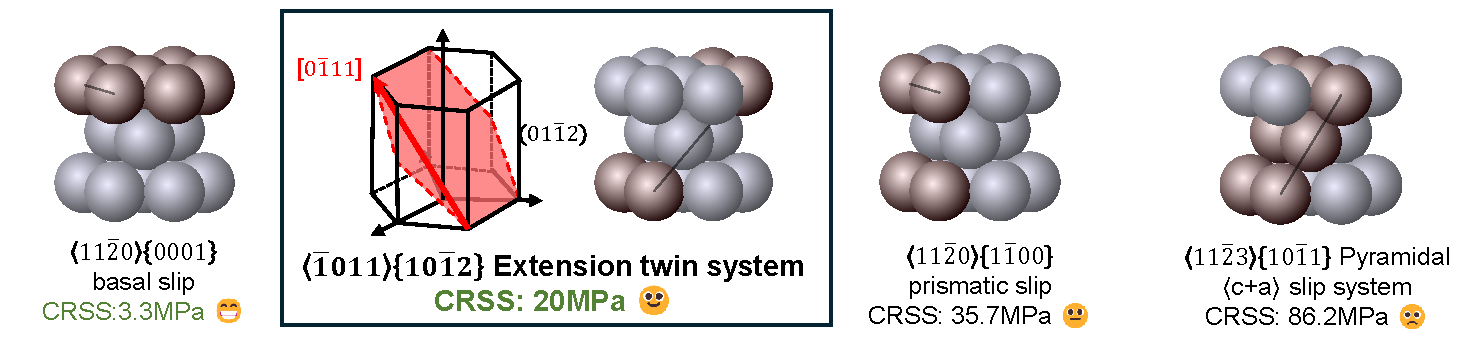
\includegraphics[width=\textwidth]{images/Mg_Deformation_systems_CRSS.pdf}
    \caption{Twin Systems and Slip Systems in Mg and CRSS values}
    \label{Twin_slip_MG_CRSS}
\end{figure}
The relative values of CRSS for slip systems and twin systems play a crucial role in determining whether twinning will contribute significantly to the plastic deformation process or not. The CRSS values for twin systems are lower than those for slip systems, hence twinning is more likely to occur and contribute to plastic deformation. Values of CRSS for different deformation modes at room temperature are given in the Table \ref{CRSS table} \cite{ARULKUMAR2016143} below for Mg\cite{Kelly19685}\cite{BEYERLEIN2011988}, Zr\cite{Knezevic201555}, Ti\cite{QIN2014293}.

\begin{table}[ht]
\centering
\caption{CRSS values of different deformation modes of HCP metals.}
\begin{tabular*}{\textwidth}
{@{\extracolsep{\fill}}c@{\extracolsep{\fill}}*{4}{@{\extracolsep{\fill}}c@{\extracolsep{\fill}}}@{\extracolsep{\fill}}}
\hline
\multicolumn{1}{c}{\textbf{Material}} & \multicolumn{4}{c}{\textbf{CRSS values of slip \& Twin modes}} \\
& Basal $\langle a\rangle$ & Prismatic $\langle a\rangle$ & Pyramidal $\langle c+a\rangle$ & T. Twin \\
\hline
Magnesium     & 3.3  & 35.7  & 86.2 & 20 \\
Zirconium     & 700  & 20    & 160  & 102 \\
Titanium     & 120  & 60    & 180  & 125 \\
\hline
\end{tabular*}

\label{CRSS table}
\end{table}

\section{Experimental observations of deformation twinning.}

\subsection{The stochastic nature of deformation twinning.}
\label{Stochastic_nature}
Beyerlein et al.  \cite{Beyerlein2010StatisticalAO} statistically analysed deformation twinning in magnesium using electron backscatter diffraction (EBSD) data. They found that twinning exhibited inherent statistical variability that could not be explained deterministically.

\begin{figure}[H]
    \centering
    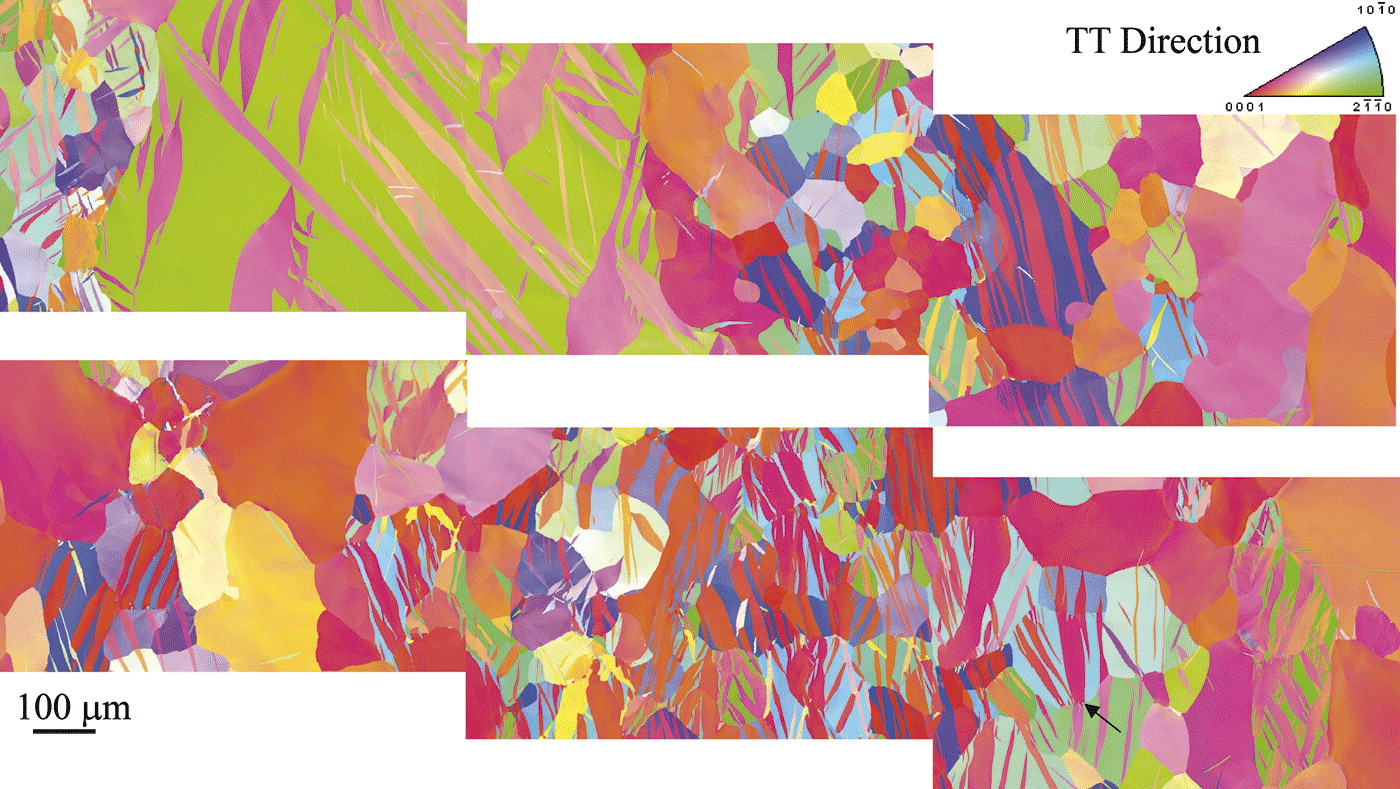
\includegraphics[width=0.7\textwidth]{images/Beyerlein_EBSD.jpg}
    \caption{ Thru-thickness EBSD orientation map of pure Mg @ 3\% compresive strain with $[1 0 \bar{1} 2]$ twinning.}
    \label{fig:8.1}
\end{figure}

Specifically, they observed that twinning occurred in some unexpectedly oriented grains, while more favourably oriented grains did not always twin. The twin variants formed also showed variability and were not always the most geometrically favoured one.

They correlated various microstructural parameters with twinning characteristics. Key findings were:
\begin{itemize}
\item Twinning did not necessarily occur in all similarly sized and oriented grains, conflicting with deterministic rules.
\item The twin variant selected was not always the one with the highest Schmid factor predicted by orientation as shown in figure \ref{fig:8.2}.
\item No clear grain size effect was found on the likelihood of twinning itself, conflicting with Hall-Petch relationships. However, the number of twins per twinned grain increased with grain size as shown in figure \ref{fig:8.2} bottom left.
\item More and thicker twins occurred at small misorientation angle grain boundaries compared to high angle boundaries as shown in figure \ref{fig:8.2} bottom right.
\item Adjoined twin pairs spanning grain boundaries grew thicker than individual twins, likely due to mutual accommodation of strain.
\end{itemize}

\begin{figure}[H]
    \centering
    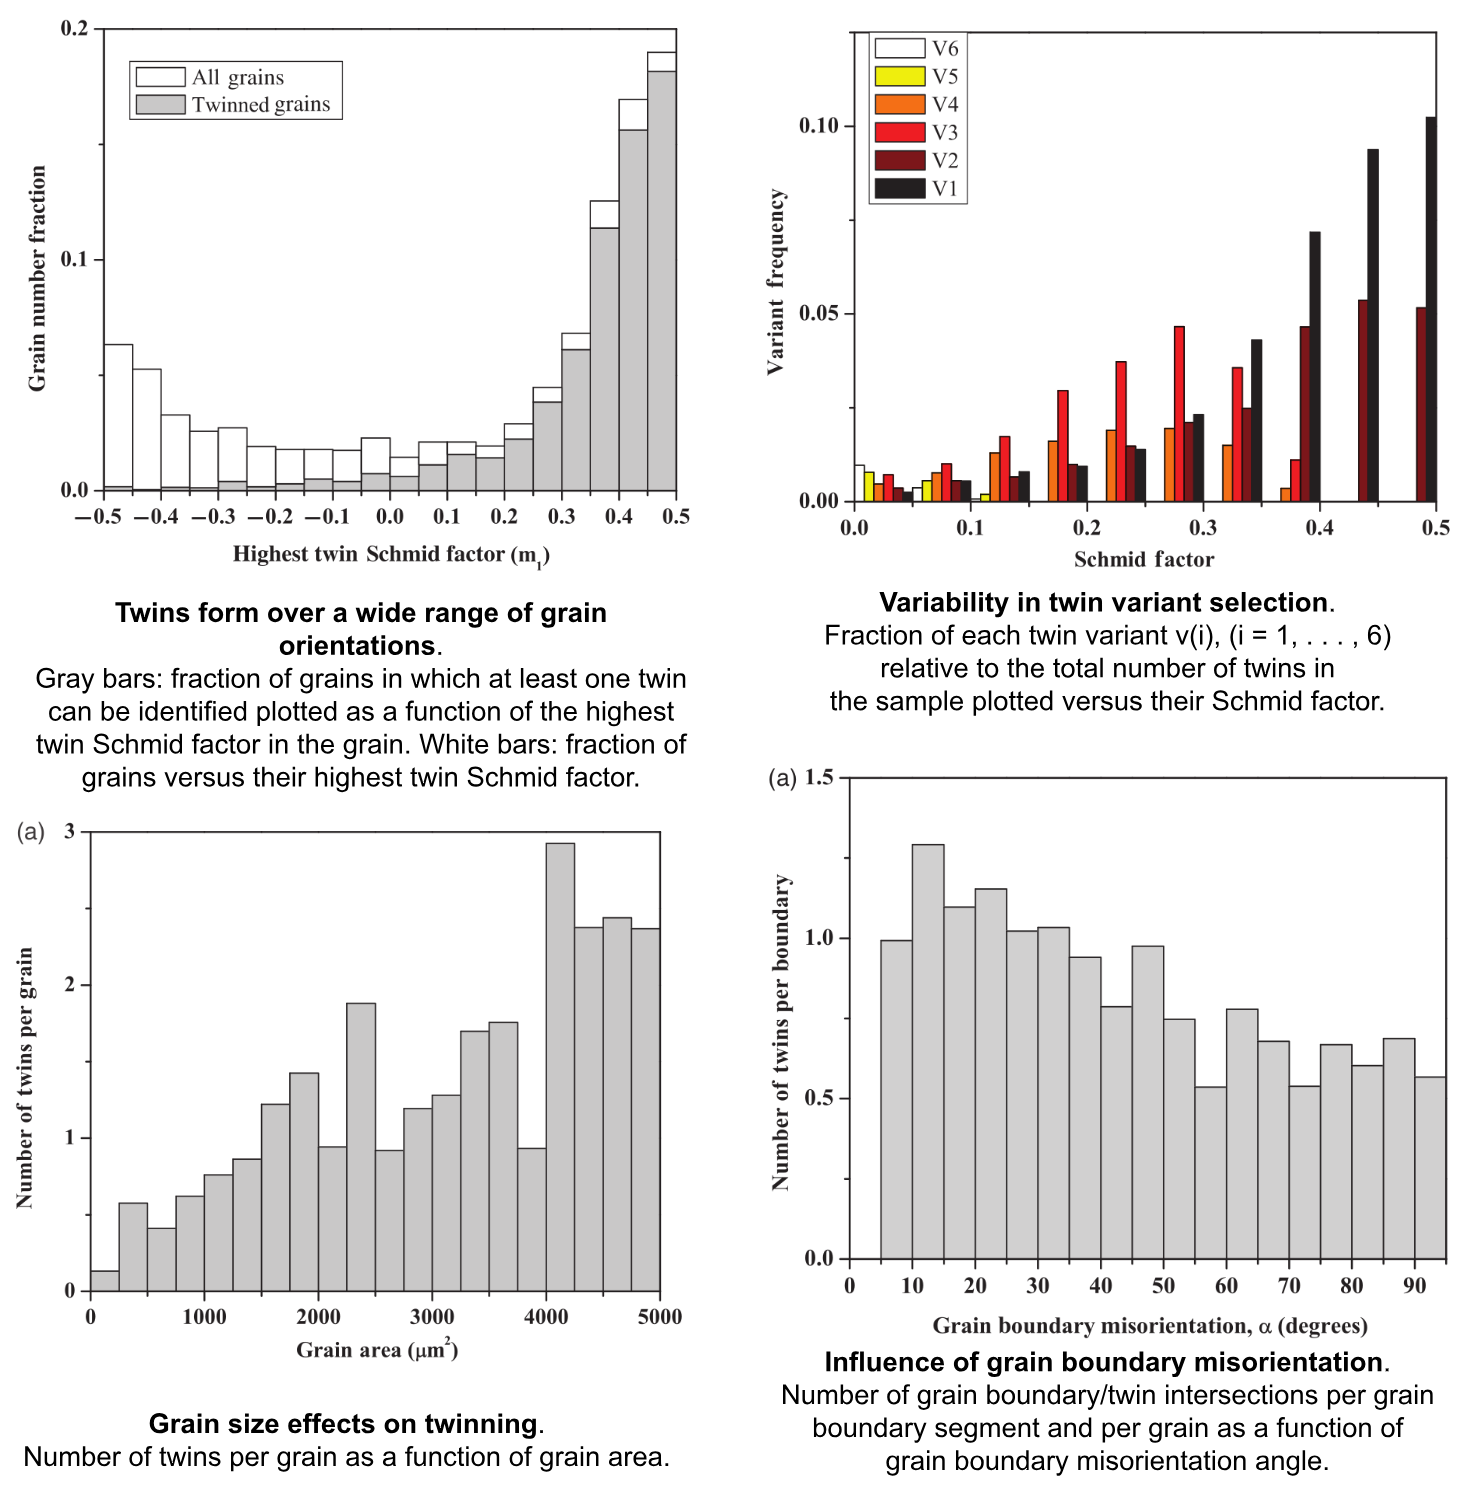
\includegraphics[width=\textwidth]{images/IB02.png}
    \caption{Effects of various crystal structure parameters on formation of twins.}
    \label{fig:8.2}
\end{figure}



\subsection{Twinning crystallography.}
\label{sec:twinning_crystallography}
Geometric description of twinning crystallography given by Christian \cite{CHRISTIAN2002859}, and recent work by Christian and Mahajan \cite{CHRISTIAN19951} is widely used to represent the twinning transformation. Here the twinning transformation is divided into four operations which preserve the symmetry.
\vspace{-0.8em}
\begin{enumerate}
    \item reflection in $K_1$,
    \vspace{-0.8em}
    \item rotation of $180^o$ about $\eta_1$,
    \vspace{-0.8em}
    \item reflection in the plane normal to $\eta_1$, and
    \vspace{-0.8em}
    \item rotation of $180^o$ about the direction normal to $K_1$
\end{enumerate}
\vspace{-0.8em}
Figure \ref{fig:Geomtery of twinning}, Geometry of twinning: We take a section of untwinned crystal sphere parallel to the plane of shear $S$. Sphere is distorted to ellipsoid due to shear $S$ along $\eta_1$ in $K_1$ plane. $\eta^{K1}$ is normal to $K_1$ plane. $K_2$ is the conjugate to the twinning plane and $\eta_2$ direction enclosed in the plane. $K_2^T$ and $\eta_2^T$ represents $K_2$ and $\eta_2$ after transformation due to twinning.

\begin{figure}[ht]
    \centering
    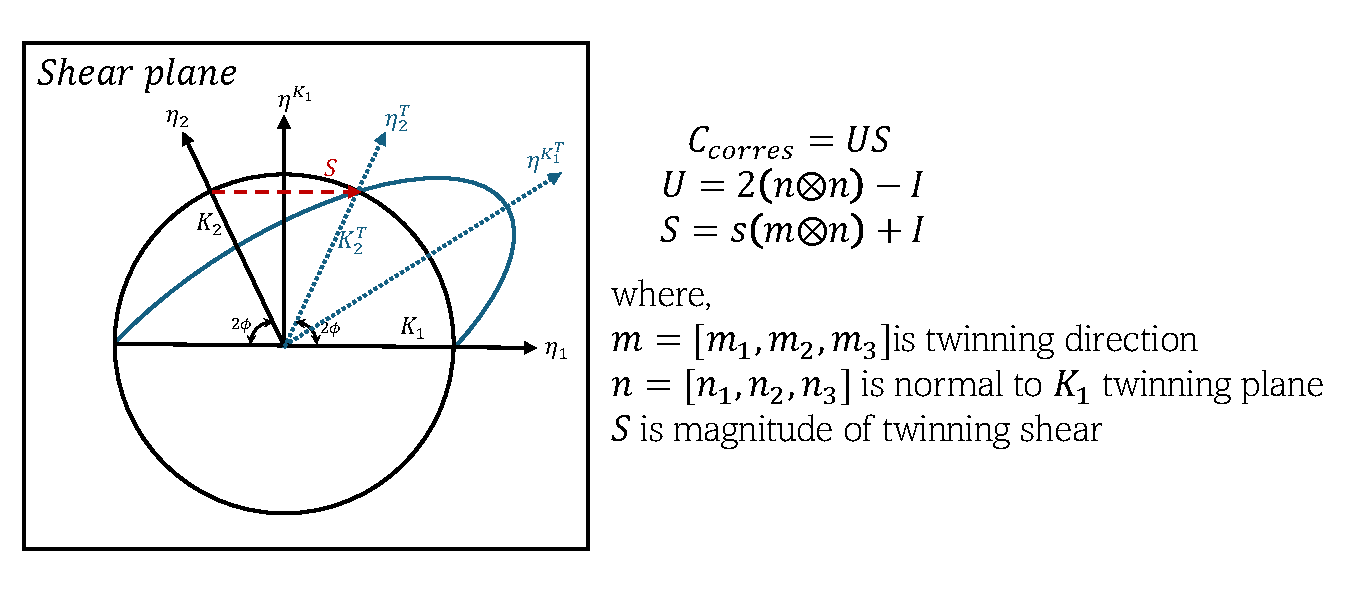
\includegraphics[width=0.95\textwidth]{images/Correspondence_matrix_theory.pdf}
    \caption{Geometrical representation of twinning.}
    \label{fig:Geomtery of twinning}
\end{figure}

\subsubsection{Quantifying the crystallographic transformation of deformation twinning in the framework of Crystal Plasticity.}

Niewczas\cite{Niewczas121} has developed deformation, re-indexation, \& correspondence matrices that quantify the lattice transformation associated with different twinning modes in hexagonal close-packed (hcp) metals. Specifically, the matrices describe the shear and rotation of lattice vectors and planes that occur when mechanical twinning operates.

These matrices can directly inform the kinematic formulations in a crystal plasticity model to capture twinning:
\begin{itemize}
\item The deformation matrix $S$ encapsulates the homogeneous shear strain produced by twinning along a specific twin mode. This defines the deformation gradient for twinning. \\ $S = s(m\otimes n)-I$ where $s$ is magnitude of twinning shear, \\ $m = [m_1,m_2,m_3] \ is \ twinning\ direction.$, and \\ $n = [n_1,n_2,n_3] \ is \ normal\ to\ K_1\ plane.$
\item The re-indexation matrix $U$ captures the crystal reorientation due to twinning. It provides the rotation component for updating the orientation of a twin domain. \\ $U = 2(n\otimes n)-I$
\item The correspondence matrix C consolidates the effects of both deformation and reorientation through twinning. C maps lattice elements from the parent to twin lattice and vice versa. \\ $C_{corres} = US$
\end{itemize}

By incorporating these transformation rules into the kinematic description, a crystal plasticity model can explicitly represent the lattice distortions that accompany the formation of a twin domain. This level of crystallographic detail enables more accurate modelling of mechanical twinning in hcp metals.

\section{Crystal plasticity models on deformation twinning.}

Over the past decades, numerous crystal plasticity models, which incorporate twinning, have been developed. However, the majority of these models have adopted a phenomenological, volume fraction-based approach to pseudo-twinning, which is spatially homogenised. While this approach may be suitable for predicting average texture and certain macroscopic properties, it has limited capability in capturing the micromechanical consequences of highly localised deformation caused by twinning, such as damage, early localization, and most importantly, the interaction between dislocation slip and twinning.

Recently, phase field modelling has demonstrated significant potential in modelling spatially resolved mechanical twinning, providing a clear interface between parent and twin orientations. However, this approach prohibitively expensive in terms of computational time and power.

Given these facts, a gap exists in the field of efficient modelling of deformation twinning using continuum approaches. Addressing this gap is essential to enhance our understanding of deformation twinning in HCP metals.

\subsection{Available crystal plasticity models for deformation twinning.}

Although twinning and slip are both responsible for plastic deformation in HCP metals. Twinning once nucleated will act at different lenghscale and timescale. Hence incorporating twinning along with slip in CP models has been always been a challenge. A chronological account of major attempts to model is presented here based on existing review article by Paudel et al \cite{Paduel202111091373}.
\vspace{-0.8em}
%Existing Crystal Plasticity Models which incorporates deformation twinning can be classified to 2 categories:
%1. Volume Fraction based approaches.
%2. Energy based and phase field approaches.
\subsubsection{1969-1978: Early attempts}
\vspace{-0.8em}
Earliest pioneering work for modelling deformation twinning was done by Chin et al. in 1969 \cite{Chin1969.0051} for cubic materials based on Taylor’s least work hypothesis\cite{taylor1938plastic}. Based on this work earliest successful simulation of deformation twinning for Brass was done by Van Houtte in 1978\cite{HOUTTE1978591} texture evolution based on the load-deformation relationship was successfully modelled for the first time. Also the concept of twinned ``\textbf{volume fraction}" was introduced for the first time. Volume fraction of twin, which is derived from the local shear stress, physically represents the fraction of twinned volume in the total volume of a specific democratized element. It is a continuous quantity which varies from 0 to 1. Volume fraction allows a discrete entity which causes discontinuity to be modelled in the continuum mechanics framework. %Additionally, in this model, they reorient the twinned grain based on Monte Carlo scheme and choose the variant of twin based on a probabilistic criteria.
\vspace{-0.8em}
\subsubsection{1991: Predominant Twin Reorientation and Volume Fraction Transfer}
\vspace{-0.8em}
Modeling deformation twinning in HCP metals was first done by Lebensohn et al. in 1991 \cite{Lebensohn1991ModellingTI}, where they improved the previous model by their ``Predominant Twinning Reorientation"(PTR) scheme which was improved again in 1991 by Tome et al.\cite{TOME19912667} when they model Zirconium. They call this as ``Volume Fraction Transfer" (VFT) scheme. These schemes use deterministic criteria where they select most dominant variant for completely(PTR) or partially(VFT) reorientation of the grain. The PTR-VFT scheme predicts texture evolution better than the the previous model.
\vspace{-0.8em}
\subsubsection{1998: Twinning as ``Pseudo Slip" in Lagrangian Framework.}
\vspace{-0.8em}
Kalidindi's Lagrangian incorporation of twinning\cite{KALIDINDI1998267} in 1998 was one of the important approaches to model the deformation twinning which is still used today in DAMASK. In this approach twinning is considered as pseudo-slip and it incorporates deformation caused by the twinning into the kinematics of the Lagrangian framework. This model is very efficient because it mainly aims to predict the stress-strain response bypassing the prediction of texture evolution.
\vspace{-0.8em}
\subsubsection{2007: Composite Grain approach}
\vspace{-0.8em}
Proust in 2007 \cite{PROUST20072137} makes an improvement for PTR-VFT scheme. In this model a crystal or grain is treated as a composite material made with matrix and twin lamellae which evolve with deformation. Here the hardening laws incorporate the twin-slip interaction making use of geometrically necessary dislocations and a directional Hall–Petch mechanism. It provides a better prediction of internal stresses and strains within a grain.
\vspace{-0.8em}
\subsubsection{2008: Dislocation-density based model}
\vspace{-0.8em}
Beyerlein and Tomé in 2008 \cite{BEYERLEIN2008867} developed a dislocation-density based model to link twinning with the evolution of dislocation density which gives a more comprehensive understanding on the effect of temperature transition from slip dominated to twinning dominated deformation.
\vspace{-0.8em}
\subsubsection{2010: Probabilistic twin nucleation model}
\vspace{-0.8em}
Beyerlein and Tomé in 2010\cite{beyerlein2010probabilistic} developed probabilistic nucleation framework to which addresses the stochastic nature of twinning. This gives much more realistic description of nucleation events leading to more accurate prediction of deformation behavior.
\vspace{-0.8em}
\subsubsection{2012: Twinning-Detwinning}
\vspace{-0.8em}
Wang et al \cite{WANG201293} proposed this model to address the detwinning behavior observed during reversed loading, which was not captured by previous models.
\vspace{-0.8em}
\subsubsection{2015-2017: Energy based approach for twin nucleation and evolution.}
\vspace{-0.8em}
This model is described in series of publications by Cheng et al.\cite{CHENG2015148}\cite{CHENG2017512}. Here energy of interactions between crystal defects are considered and energy for dislocation dissociation is considered as nucleation criteria. Twin propagation is based on thermal energy calculated from shearing and shuffling of atoms. 
\vspace{-0.8em}
\subsubsection{2014-2021: Phase Field Twinning Model}
\vspace{-0.8em}
In this very recent approach by Kondo et al. 2014 \cite{KONDO2014672} and Liu et al.  Twin and parent regions are treated as different phases described by an order parameter $\eta$. Stochastic methods are used for twin nucleation mechanism and the evolution of the twin order parameter driven by discrete twin interface energy. This enables modeling of complex twin morphologies and their interactions with other microstructural defects.

\vspace{0.5em}
These models can be broadly classified to two groups:
\vspace{-0.8em}
\begin{enumerate}
    \item Volume fraction based approaches.
    \vspace{-0.8em}
    \item Energy based or phase field approaches.
\end{enumerate}
%\vspace{-0.8em}
Volume fraction based approaches have been less accurate to predict either texture evolution or load-deformation response, and Energy based or phase field approaches have been less computationally efficient.

The table \ref{Comparision of CP models for twinning} gives the summary of all the literature regarding different Crystal Plasticity models which were reviewed for this work.


\begin{table}[H]
  \centering
  \caption{Comparision of different CP models for twinning.}
  \renewcommand\arraystretch{1.2}
  \renewcommand\baselinestretch{1.2}
  \begin{tabular}{|m{4.2cm}|m{7.8cm}|c|}
    \hline
    CP Model & Model Features & Remarks \\
    \hline
    Predominant twin reorientation \cite{HOUTTE1978591} & Predicts texture evolution using predominant twin system & \multicolumn{1}{|c|}{\multirow{15}{2cm}{Volume Fraction based, less accurate}} \\
    \cline{1-2}
    Volume Fraction Transfer \cite{TOME19912667} & PTR + volume fraction variable for accurate prediction of texture. & \multicolumn{1}{|c|}{} \\
    \cline{1-2}
    Kalidindi's Lagrangian method.\cite{KALIDINDI1998267} & Incorporates twinning as ``pseudo-slip" in kinematics based on evolution of volume fraction. & \multicolumn{1}{|c|}{} \\
    \cline{1-2}
    Updated Lagrangian method \cite{LEVESQUE201065} \cite{Lebensohn.2003.1212} & Also incorporates secondary twins and slips and tertiary slip. & \multicolumn{1}{|c|}{} \\
    \cline{1-2}
    Composite Grain model \cite{PROUST20072137} \cite{PROUST2009861} & Incorporates effect of SSD, GND and Hall-Petch effect at twin interfaces. & \multicolumn{1}{|c|}{} \\
    \cline{1-2}
    Twinning detwinning model \cite{WANG201293} \cite{WANG201336} & Incorporates detwinning in a CP model to simulate hysteresis & \multicolumn{1}{|c|}{} \\
    \cline{1-2}
    Dislocation-density based model \cite{BEYERLEIN2008867} \cite{Knezevic201555} & Includes dislocation transmutation and twin accommodation effects to predict plastic anisotropy. & \multicolumn{1}{|c|}{} \\
    \cline{1-2}
    Probabilistic nucleation method \cite{beyerlein2010probabilistic} \cite{BARNETT2015151} & Based on numerical observation from atomistic simulations and statistical analyses. & \multicolumn{1}{|c|}{} \\
    \cline{1-2}
    Explicit incorporation method \cite{ABDOLVAND2013783} \cite{ARDELJAN2015396} & Twin is explicitly incorporated by remeshing RVE before every timestep to achieve spatially resolved fields & \multicolumn{1}{|c|}{} \\
    \hline
    Energy based micro-twin nucleation model \cite{CHENG2015148} \cite{PARAMATMUNI2020102778} & Based on energy of dislocation interaction. Predicts heterogeneous twin formation with strain localization. & \multicolumn{1}{|c|}{\multirow{3}{2cm}{Energy based approaches, Computationally expensive}} \\
    \cline{1-2}
    Thermal activation based twin propagation method \cite{CHENG2017512} \cite{Ghosh2018} & Nucleation based on thermal energy activation which accounts for shear-shuffle process. & \multicolumn{1}{|c|}{} \\
    \cline{1-2}
    Phase field twinning model \cite{KONDO2014672} \cite{GRILLI2020104061} & Twin evolution as a phase transformation of parent into twin. Based on Gibbs energy. & \multicolumn{1}{|c|}{} \\
    \hline
  \end{tabular}
  \label{Comparision of CP models for twinning}
\end{table}

\section{Software for Crystal Plasticity modeling and simulation.}
There are many software available to create constitutive models and run simulations. Based on license we can classify them as commercial and open source.

List of some commercial software:
\vspace{-0.8em}
\begin{itemize}
    \setlength\itemsep{-0.5em}
    \item ABAQUS
    \item ANSYS
    \item MSC(MARC)
    \item COMSOL
\end{itemize}
\vspace{-0.8em}
List of some opensource software:
\vspace{-0.8em}
\begin{itemize}
    \setlength\itemsep{-0.5em}
    \item DAMASK
    \item PRISMS
    \item MOOSE
    \item FEniCS
    \item FreeFEM
\end{itemize}

For the choice of implementation of our model we compare various software available to us as given in the table \ref{CP-Software-Comparision}.

\begin{table}[H]
\centering
 \caption{Comparison of some notable software used for Crystal Plasticity Simulations.}
\begin{tabular}{ |m{4.3em}||m{4.2cm}|m{2.5cm}|m{1.7cm}|m{2.7cm}| }
 \hline
 & \multicolumn{4}{|c|}{Features} \\
 \hline
 Software& Developer(s) & License & Language & Solver Choices \\
 \hline \hline
 DAMASK &Max-Planck-Institut für Eisenforschung GmbH&Open Source&Fortran& FFT and FEM \\ %(Implicit)
 \hline
 ABAQUS&Dassault Systèmes&Proprietary /commercial&Fortran&FEM \\ %(Implicit and Explicit)
 \hline
 MOOSE &Idaho National Lab&Partially Open Source&C++&FEM \\ %(Implicit and Explicit)
 \hline
 PRISMS / deal.II&University of Michigan / Universität Heidelberg&Open Source&C++& FEM \\ %(Implicit and Explicit)
 \hline
 FEniCS &(Multiple) &Open Source&C++ \& Python& FEM \\ %(Implicit and Explicit)
 %\hline
 %WARP3D&University of Illinoi&Open Source & FEM\\
 \hline
\end{tabular}

 \label{CP-Software-Comparision}
 \end{table}
 
\subsubsection{The choice of DAMASK.}
From the review of different software packages available, we make an informed choice for implementing our discrete twin model. DAMASK is chosen as it gives choice of 2 solvers to test our model. DAMASK is modular and implementation of our model does not affect the other components of the code. At the same time DAMASK integrates all the modules such that it gives access to most internal subroutines and functions, the state container to store and manipulate results, and neighbouring elements or integration points. We utilize these features in our model.

\section{DAMASK.}
DAMASK (Düsseldorf Advanced Material Simulation Kit) \cite{ROTERS2019420}, an open source software developed by the Max-Planck-Institut für Eisenforschung, to implement our discrete twin model due to its powerful capabilities in multi-physics crystal plasticity simulations. One of the key advantages of DAMASK is that it is open source, allowing us to directly access and modify the source code to build customized features and models into the software.

\subsection{Concept:}
DAMASK provides tools to solve the constitutive response that connects deformation and stress at each material point based on Crystal Plasticity using a variety of constitutive models and homogenization approaches. DAMASK is capable of handling multi-physics problems, following a modular approach, additional field equations containing displacive phase transformation, significant heating, and potential damage evolution are solved in a fully coupled way. 

DAMASK was developed to emulate the multi-scale hierarchy and multi-physics structure observed in the material physics of thermo-mechanical loading of complex materials. Consequently, it defines template functions that link numerical solvers, homogenization methods, and constitutive laws. To increase flexibility, one can combine various constitutive laws and homogenization schemes, along with a specific set of solvers for the associated boundary and/or initial value issues, in the same model.
\subsubsection{Hierarchical structure of different modules:}
Damask is a modular software with a hierarchical structure
\begin{figure}[H]
    \centering
    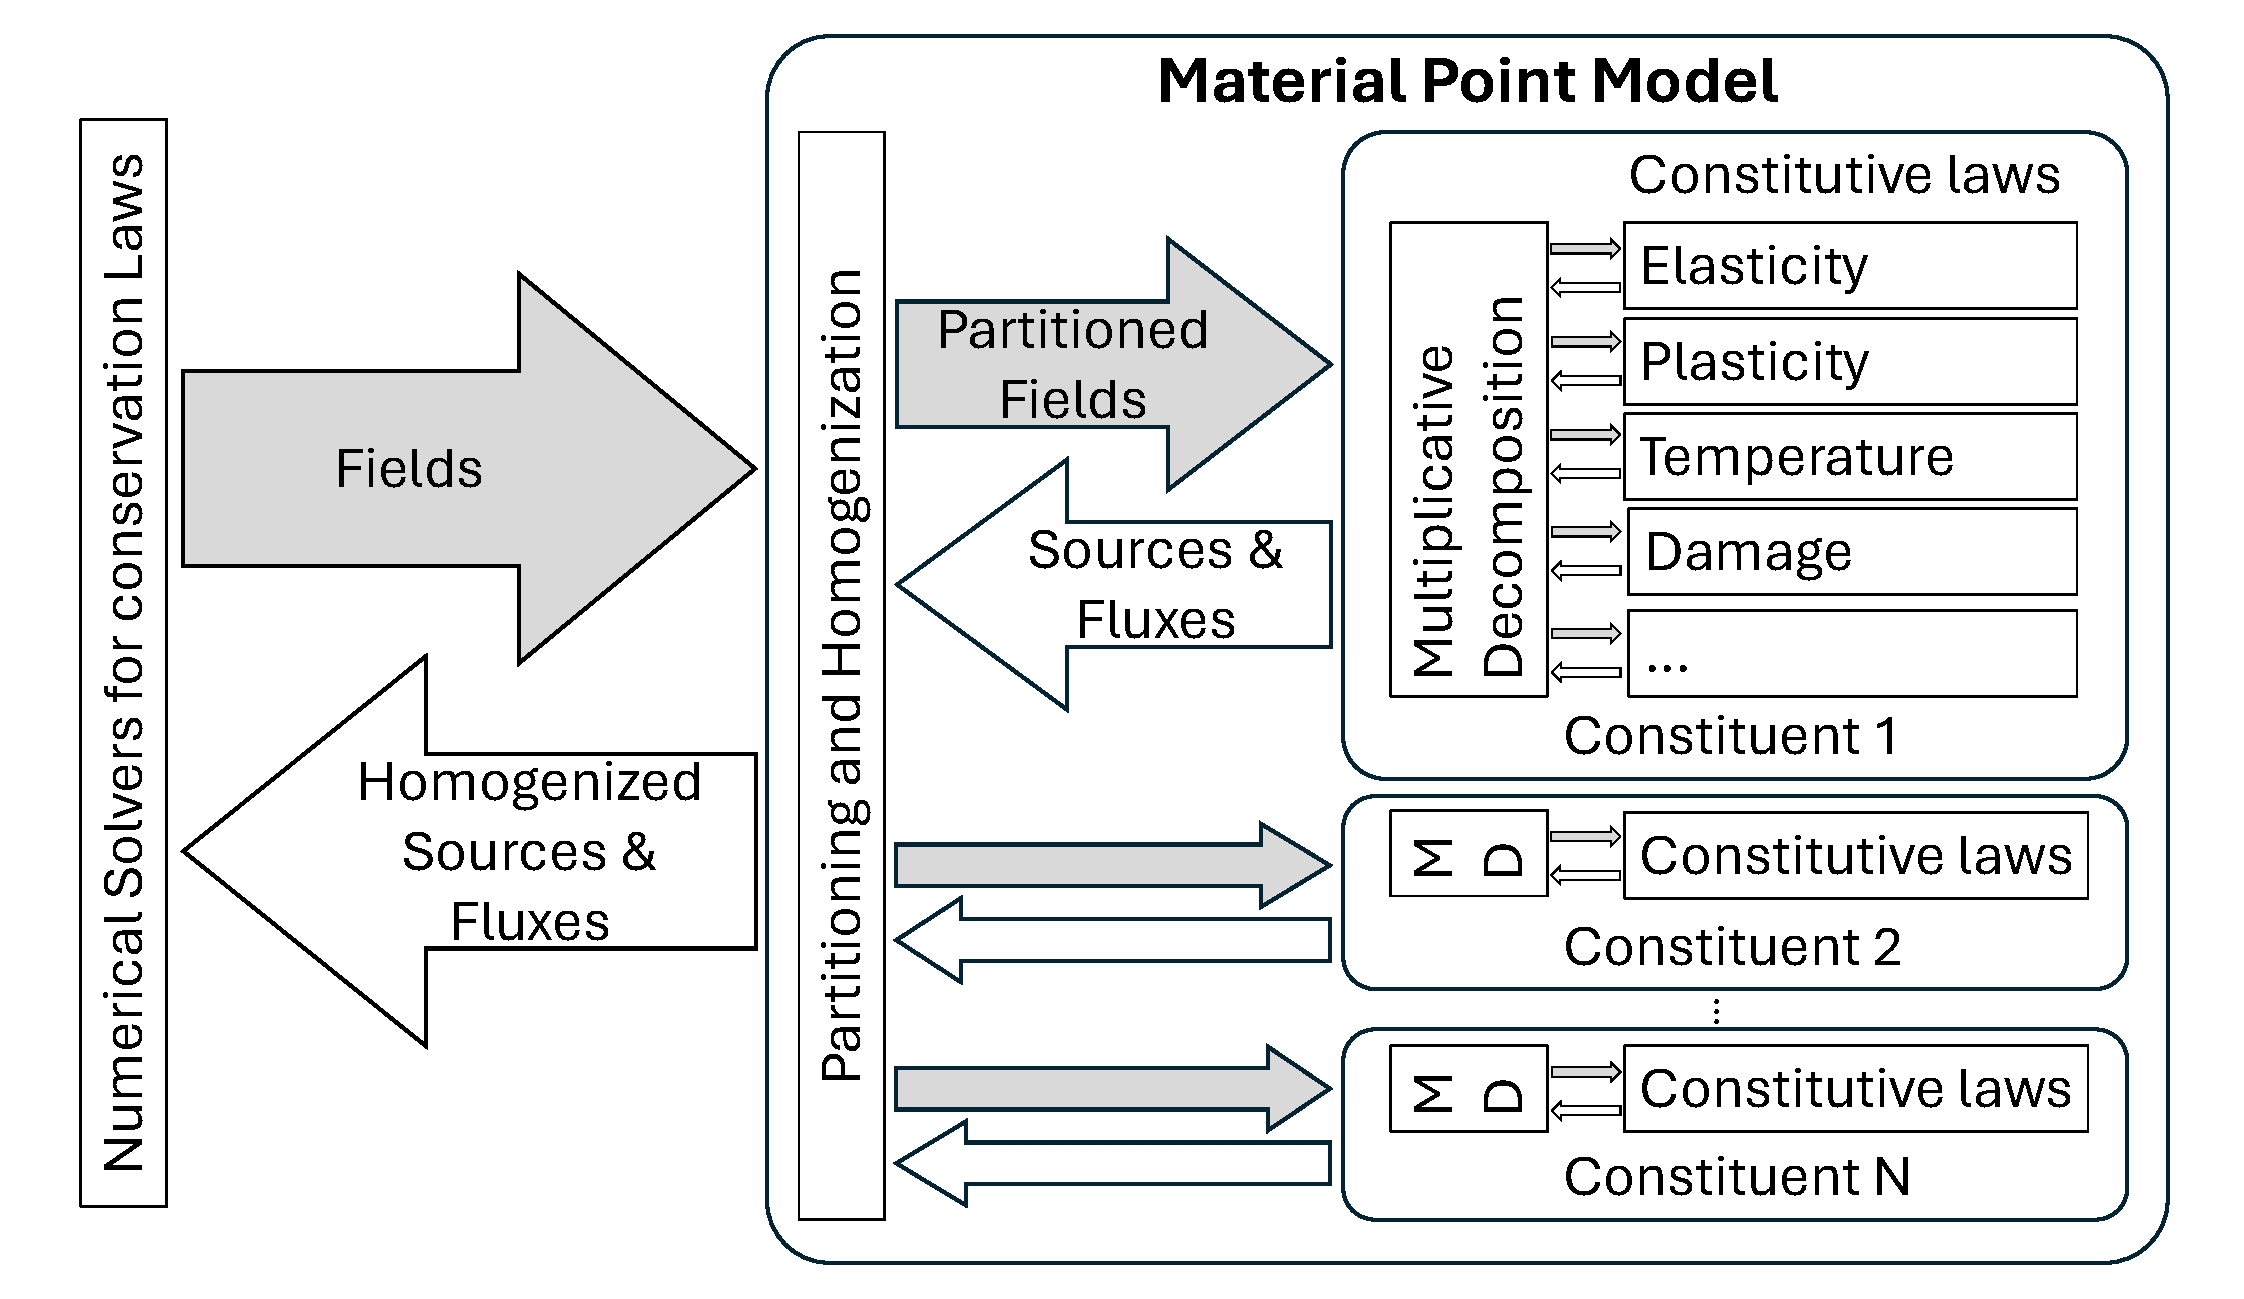
\includegraphics[width=\textwidth]{images/Hierarchical structure of DAMASK at a material point.pdf}
    \caption{Hierarchical structure of DAMASK at a material point}
    \label{DAMASK_hierarchy}
\end{figure}


The conservation laws in DAMASK require a structured multi-scale description of the fluxes and sources across hierarchical levels. At the highest level, a division and homogenization scheme partitions prescribed field values on a material point among its underlying microstructural elements and subsequently homogenizes each constituent's constitutive reaction. At the intermediate Constituent Level, time integration of the underlying constitutive laws determines the reaction of each microstructural constituent in terms of fluxes and sources. Finally, at the lowest level, constitutive laws based on evolving internal state variables provide this response.
\subsection{Constitutive Models:}
Constitutive models form the foundational blocks of DAMASK's hierarchical structure, characterized by internal state variables that capture history dependence.
\subsubsection{Elasticity}
The elastic behavior is modeled using a Generalized Hooke's Law that relates the Second Piola-Kirchhoff stress $S$ and Green-Lagrange strain $E$ through an elastic stiffness matrix $\mathbb{C}$. 
\begin{equation}
    S = \mathbb{C} : E\
\end{equation}
\subsection{Plasticity:}
The crystal plasticity laws provide the plastic velocity gradient $L_p$ for a given Mandel stress $M_p$.
\subsubsection{Phenomenological Crystal Plasticity in DAMASK:}
In polycrystalline materials, plastic deformation occurs on well-defined planes and directions dictated by the lattice structure. The total plasticity is calculated as the sum of the shear rates from the individual slip systems according to the following equation:
\begin{equation}
    L_p = \sum_{\alpha} \dot{\gamma} ^\alpha \underbrace{(s_{S}^{\alpha} \otimes n_{S}^{\alpha})}_{=:P_{Schmid}^{\alpha}}
\end{equation}
s and n are the directions and Normal's to the slip planes. Schmid's law provides the expression for the resolved shear stress which acts as driving force for plastic slip:
\begin{equation}
 \tau^\alpha=M_p . P_{Schmid}^{\alpha}
\end{equation}
The modified form of Phenomenological Crystal Plasticity introduced by Hutchinson for FCC and extended to twinning by Kalidindi is used in DAMASK. The plastic component in the internal variables represents resistances to slip and twinning. It is characterized by the equation:
\begin{multline}
\dot{\xi}^{\alpha}=h_{0}^{s-s}(1+c_1(f_{tw}^{tot})^{c_2})(1+h_{int}^{\alpha}) \\ *
\sum_{\alpha'=1}^{N_s} \lvert\dot{\gamma}^{\alpha'}\rvert \bigg|1-\frac{\dot{\xi}^{\alpha'}}{\dot{\xi}^{\alpha'}_{\infty}}\bigg|^{\alpha} sign\bigg(1-\frac{\dot{\xi}^{\alpha'}}{\dot{\xi}^{\alpha'}_{\infty}}\bigg)h^{\alpha\alpha'}+\sum_{\beta'=1}^{N_tw} \dot{\gamma}^{\beta'}h^{\alpha\beta'}
\end{multline}
Where $f_tot_tw$ represents the twin volume fraction and h covers the slip-slip and slip-twin interaction parameters. The remaining terms are model fitting parameters. Likewise, the evolution of resistances on twin systems is given by:
\begin{equation}
\dot{\xi}^{\beta}=h_{0}^{tw-s}(\sum_{\alpha=1}^{N_s}\lvert\dot{\gamma}^{\alpha}\rvert)^{c_3} \sum_{\alpha'=1}^{N_s}\lvert\dot{\gamma}^{\alpha'}\rvert h^{\beta\alpha'} + h_{0}^{tw-tw} (f_{tw}^{tot})^{c_4}  \sum_{\beta'=1}^{N_tw} \dot{\gamma}^{\beta'}h^{\beta\beta'}
\end{equation}

The evolution of shear rate on each slip system is given by,

\begin{equation}
\dot{\gamma}^{\alpha} = (1-f_{tw}^{tot}) \dot{\gamma}^{\alpha}_{0} \bigg| \frac{\tau^\alpha} {\xi^\alpha} \bigg|^n sgn(\tau^\alpha)
\end{equation}

The evolution of shear rate due to mechanical twinning takes into account the unidirectional character of twin formation:

\begin{equation}
\dot{\gamma} = (1-f_{tw}^{tot}) \dot{\gamma}_{0} \bigg| \frac{\tau}{\xi} \bigg|^n \mathcal{H}(\tau^\alpha)
\end{equation}

where $\mathcal{H}$ is the heaviside or unit step function. The total twin volume fraction is given by,

\begin{equation}
f_{tw}^{tot} = max \left(  \sum_{\beta=1}^{N_{tw}} \underbrace{\frac{\gamma^{\beta}}{\gamma^{\beta}_{char}}}_{=:f^{\beta}_{tw}},1.0 \right)
\end{equation}
where $\gamma_{char}$ is the characteristic shear dye to mechanical twinning, the value of which depends on the twin system.

%dgmdt(is) = shrt_0*abs(tau_eff(is)/IVB_eff(is)))**pw_fl*sign(1.d0,tau_eff(is))

%This behavior is described by the constitutive equation \eqref{eq:shear_strain_rate}

%\eqref{eq:shear_strain_rate}

%\begin{equation}
%\dot{\gamma} = \dot{\gamma}_{0} \left| \frac{\tau_{eff}}{\tau_{Ceff}} \right|^n \operatorname{sign}(\tau_{eff})
%\end{equation}

% ddgmdt_dtau(is) = pw_fl/IVB_eff(is)*shrt_0*(abs(tau_eff(is)/IVB_eff(is)))**(pw_fl-1)

%\begin{equation}
%    \frac{\dot{\gamma}}{\dot{\tau}} = \frac{n}{\tau_{eff}} \dot{\gamma}_{0} 
%\end{equation}

%\begin{equation}
%\dot{\gamma} = \dot{\gamma}_{0} \left| \frac{\tau_{eff}}{\tau_{Ceff}} \right|^n \operatorname{sign}(\tau_{eff}) \label{eq:shear_strain_rate}
%\end{equation}

% ddgmdt_dIVB(is) = -pw_fl*dgmdt(is)/IVB_eff(is)

% ddIVBdt_dIVB(is,js) = crsF_mat(is,js)*hdrt_0*ddgmdt_dIVB(js)*sign(1.d0,tau_eff(js))*x1**pw_hd - crsF_mat(is,js)*hdrt_0*abs(dgmdt(js)) *x1**(pw_hd-1)*pw_hd/crss_s
